\chapter{Microfrontend}\label{ch:chapter1}
\begin{figure}[H]
  \centering
  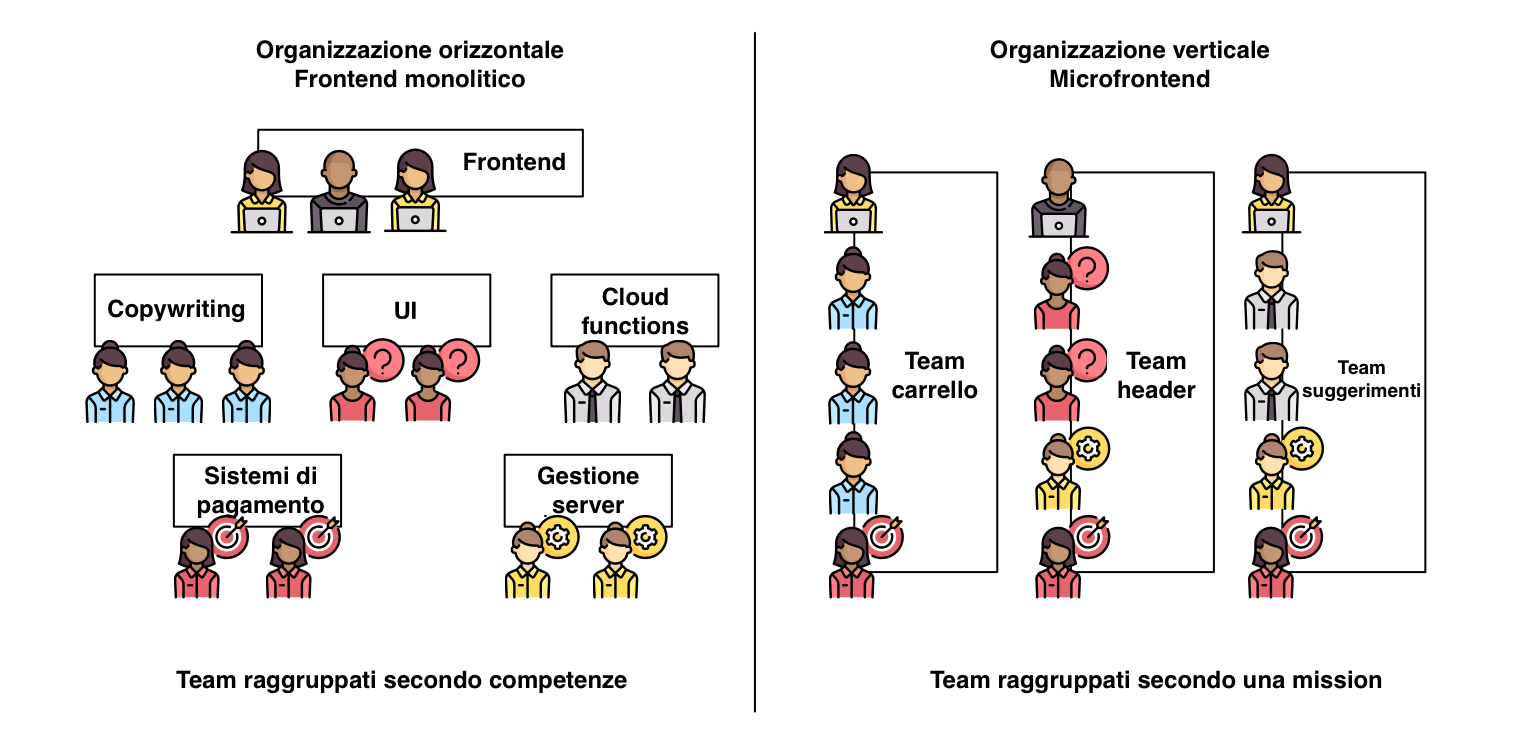
\includegraphics[width=140mm]{img/schema_microfrontend}
  \caption{Differenze di composizione di team tra approccio monolitico e microfrontend}
\end{figure}
L'obiettivo della tecnologia microfrontend è quello di superare l'approccio monolitico, che vede
lo sviluppo di applicazioni web suddiviso in due team: backend e frontend.
\\
Possiamo considerare un'applicazione web come un insieme
di elementi, chiamati fragment o microfrontend, disaccoppiati tra di loro
e con la più bassa granuralità, ovvero con la funzionalità più minimale possibile.
\\Ogni microfrontend viene sviluppato da un team, che potrà lavorare con autonomia. 
Essendo i singoli microfrontend autonomi,
questi possono funzionare anche se estratti dalla applicazione web che li contiene,
 e il malfunzionamento di un singolo microfrontend
non compromette la stabilità degli altri.
I team sono autonomi, ma non sono isolati: questi infatti condividono un insieme di dati, che
chiameremo \emph{contratto},
fondamentali per il corretto funzionamento dell'applicazione. A seconda delle tecnologie utilizzate
per realizzare l'architettura microfrontend, il contratto tra i team sarà più o meno complesso.

\section{Vantaggi}
\begin{itemize}
    \item \textbf{Ottimizzare lo sviluppo di funzionalità:}
Nell’approccio orizzontale quando si vuole sviluppare una nuova funzionalità è necessario far convergere il 
lavoro di più team. Con microfrontend,
  tutte le persone coinvolte nell’implementazione di una nuova funzionalità sono nello 
  stesso team, rendendo il lavoro più veloce ed efficiente. 
    \item \textbf{Verticalizzazione dei team:}
Con microfrontend le applicazioni, incluse il frontend, si dividono in sistemi verticali
 più piccoli. Ogni team controlla la sua piccola parte di frontend e di backend.
    \item \textbf{Adottare diverse tecnologie:}
Strumenti di sviluppo e framework evolvono continuamente. Ogni team deve essere in grado di scegliere
le proprie tecnologie autonomamente. Ci sono alcune grandi aziende
 come Github, che hanno
 impiegato molto tempo per eliminare alcune dipendenze ormai obsolete dal loro codice (nel caso di Github si trattava di una versione di JQuery).
  Con l’approccio microfrontend questi cambiamenti sono più rapidi e possono essere
   fatti modularmente.

\item \textbf{Indipendenza:}
I progetti di ogni team sono autonomi, ovvero non hanno dipendenze condivise tra di loro.\\
L’indipendenza però porta sicuramente a costi aggiuntivi. Si potrebbe pensare che sia
 più semplice quindi di sviluppare un unico progetto, e assegnare parti di questo a team diversi. 
 Il problema sta nel fatto che la comunicazione tra i vari team è costosa e porta molti ritardi.
In alcuni casi quindi è preferibile introdurre ridondanza nel codice dei vari team a favore di più autonomia e velocità di
 implementazione.

\end{itemize}

\section{Svantaggi}
\begin{itemize}

\item \textbf{Ridondanza:}
In informatica si è addestrati a ridurre al minimo le ridondanze.
Anche nel caso dello sviluppo frontend ci sono degli episodi nei quali la ridondanza può
 essere molto costosa: come ad esempio quando viene trovato un bug in una libreria e 
 questo viene risolto da un team, il fix dovrà essere comunicato agli altri e questi 
 dovranno provvedere a risolverlo autonomamente. Oppure quando si rende un processo più 
 veloce, anche in questo caso va comunicato agli altri team e questi dovranno apprendere
  la scoperta.
Si adotta quindi un approccio microfrontend quando i costi associati a ridondanze sono 
inferiori agli impatti negativi a uno sviluppo frontend monolitico, che porta a forti 
dipendenze tra team.




\item \textbf{Inconsistenza:}
 Potrebbero essere presenti delle basi di dati, necessarie all'applicazione web, che vengono lette e scritte
 da più microfrontends.
Per garantire la proprietà di indipendenza tra team è necessario replicare il database per tutti i progetti. 
Tutte queste copie devono però essere sincronizzate tra loro regolarmente per mantenere la consistenza e la coerenza dei dati.
Questo introduce dei ritardi, che potrebbero penalizzare l'esperienza utente.

\item \textbf{Eterogeneità:}
Potrebbe essere controverso avere la libertà di utilizzare tecnologie diverse tra i vati team.
 Ovviamente se ogni team usa una diversa tecnologia lo scambio di pareri o di competenze 
 tra team diventa più difficile.
\end{itemize}